\documentclass[../../main.tex]{subfiles}

\begin{document}

\section{Introduction}

Neural Process (NP) is a meta-learning framework introduced in \cite{garnelo2018neural, garnelo2018conditional} that can be used for few-shot uncertaincy aware meta learning. There exists two variants of the Neural Process, the Conditional Neural Process (CNP) and the Latent Neural Process (LNP), whilst we will discuss the differences between the two in this chapter, we will focus on the CNP for the majority of the project and hence we will implicitly refer to CNP as NP. 

The main idea behind Neural Processes is to learn a distribution over the target points conditioned on the context points. Context points are the input-output pairs that the model is trained on and is used to condition the model to predict the target points, which are the input locations we want to predict the output for. The model is trained on a sets of context-target pairs and then tested on a new set of context-target pairs to see how well it can generalize to new tasks. 

% \section{Neural Processes}

% Neural Processes are an expansion of Gaussian Processes using Neural Networks introduced in \cite{garnelo2018neural} they are trained on a context dataset which is. Neural processes are a meta-learning algorithm that can be used for few-shot learning. They are trained on a context dataset which is a set of input-output pairs $\mathcal{D} = \{ (x_i, y_i) \}_{i=1}^N$. 

% \subsection{Meta Learning}

% Meta-Learning is a method of ML where the model is trained on a set of tasks and then tested on a new task. The goal is to learn a model that can learn new tasks quickly`', i.e. `learning to learn'. These come under the terminology of few-shot learning where the model is trained on a small number of examples (more specifically, we can say $N$-way-$K$-shot learning where $N$ is the number of classes and $K$ is the number of examples per class).

% Consider a set of datasets $\mathcal{D} = \{ \mathcal{D}_i \}_{i=1}^D$ where each dataset $\mathcal{D}_i$ is a set of input-output pairs $\mathcal{D}_i = \{ (x_{ij}, y_{ij}) \}_{j=1}^{N_i}$. The goal of meta-learning is to learn a model $f$ that can learn a new task $\mathcal{D}_{N+1}$ with a small number of examples, i.e. few-shot learning.

\section{Architecture}

A meta-dataset is split into two sets, the context set and the target set (also called the query set) where the sets are disjoint $\mathcal{D} = \mathcal{C} \cup \mathcal{T}$ and $\mathcal{C} \cap \mathcal{T} = \emptyset$. The model is trained on the context set and then tested on the target set to see how well it can generalize to new tasks. In essence, our task is to predict the outputs for the target conditioned on the training of the context set.

To achieve this we used a neural network (usually MLP) to encode the context set into embeddings. 

\begin{equation}
    \bm{r}(\mathcal{C}_i) = \text{Enc}_\theta(\mathcal{C}_i) = \text{Enc}_\theta(\{ \bm{x}_{i}\isup{c}, \bm{y}_i\isup{c} \})
\end{equation}

Where $\bm{r}$ is the embedding of the context set $\mathcal{C}_i$ and $\theta$ are the parameters of the encoder. Then we aggregate the embeddings of the context sets to get a global representation of the dataset. 

\begin{equation}
    \bm{R}(\mathcal{C}) = \text{Agg}(\{ \bm{r}(\mathcal{C}_i) \}_{i=1}^D)
\end{equation}

Typically the aggregation function is a simple summation of the embeddings. The global representation $\bm{R}$ is then used to condition the decoder to predict the outputs of the target set $\mathcal{T} = \{ \bm{x}_{i}\isup{t} \}$ to give us a posterior distribution over the outputs $\bm{y_i\isup{t}}$.

\begin{equation}
    p(\bm{y}_i\isup{t} | \bm{x}_i\isup{t}, \mathcal{C}) = \text{Dec}_\theta(\bm{x}_i\isup{t}, \bm{R}(\mathcal{C}))
\end{equation}

The overall architecture is shown in Figure \ref{fig:cnp-architecture}.

\begin{figure}[H]
	\centering
	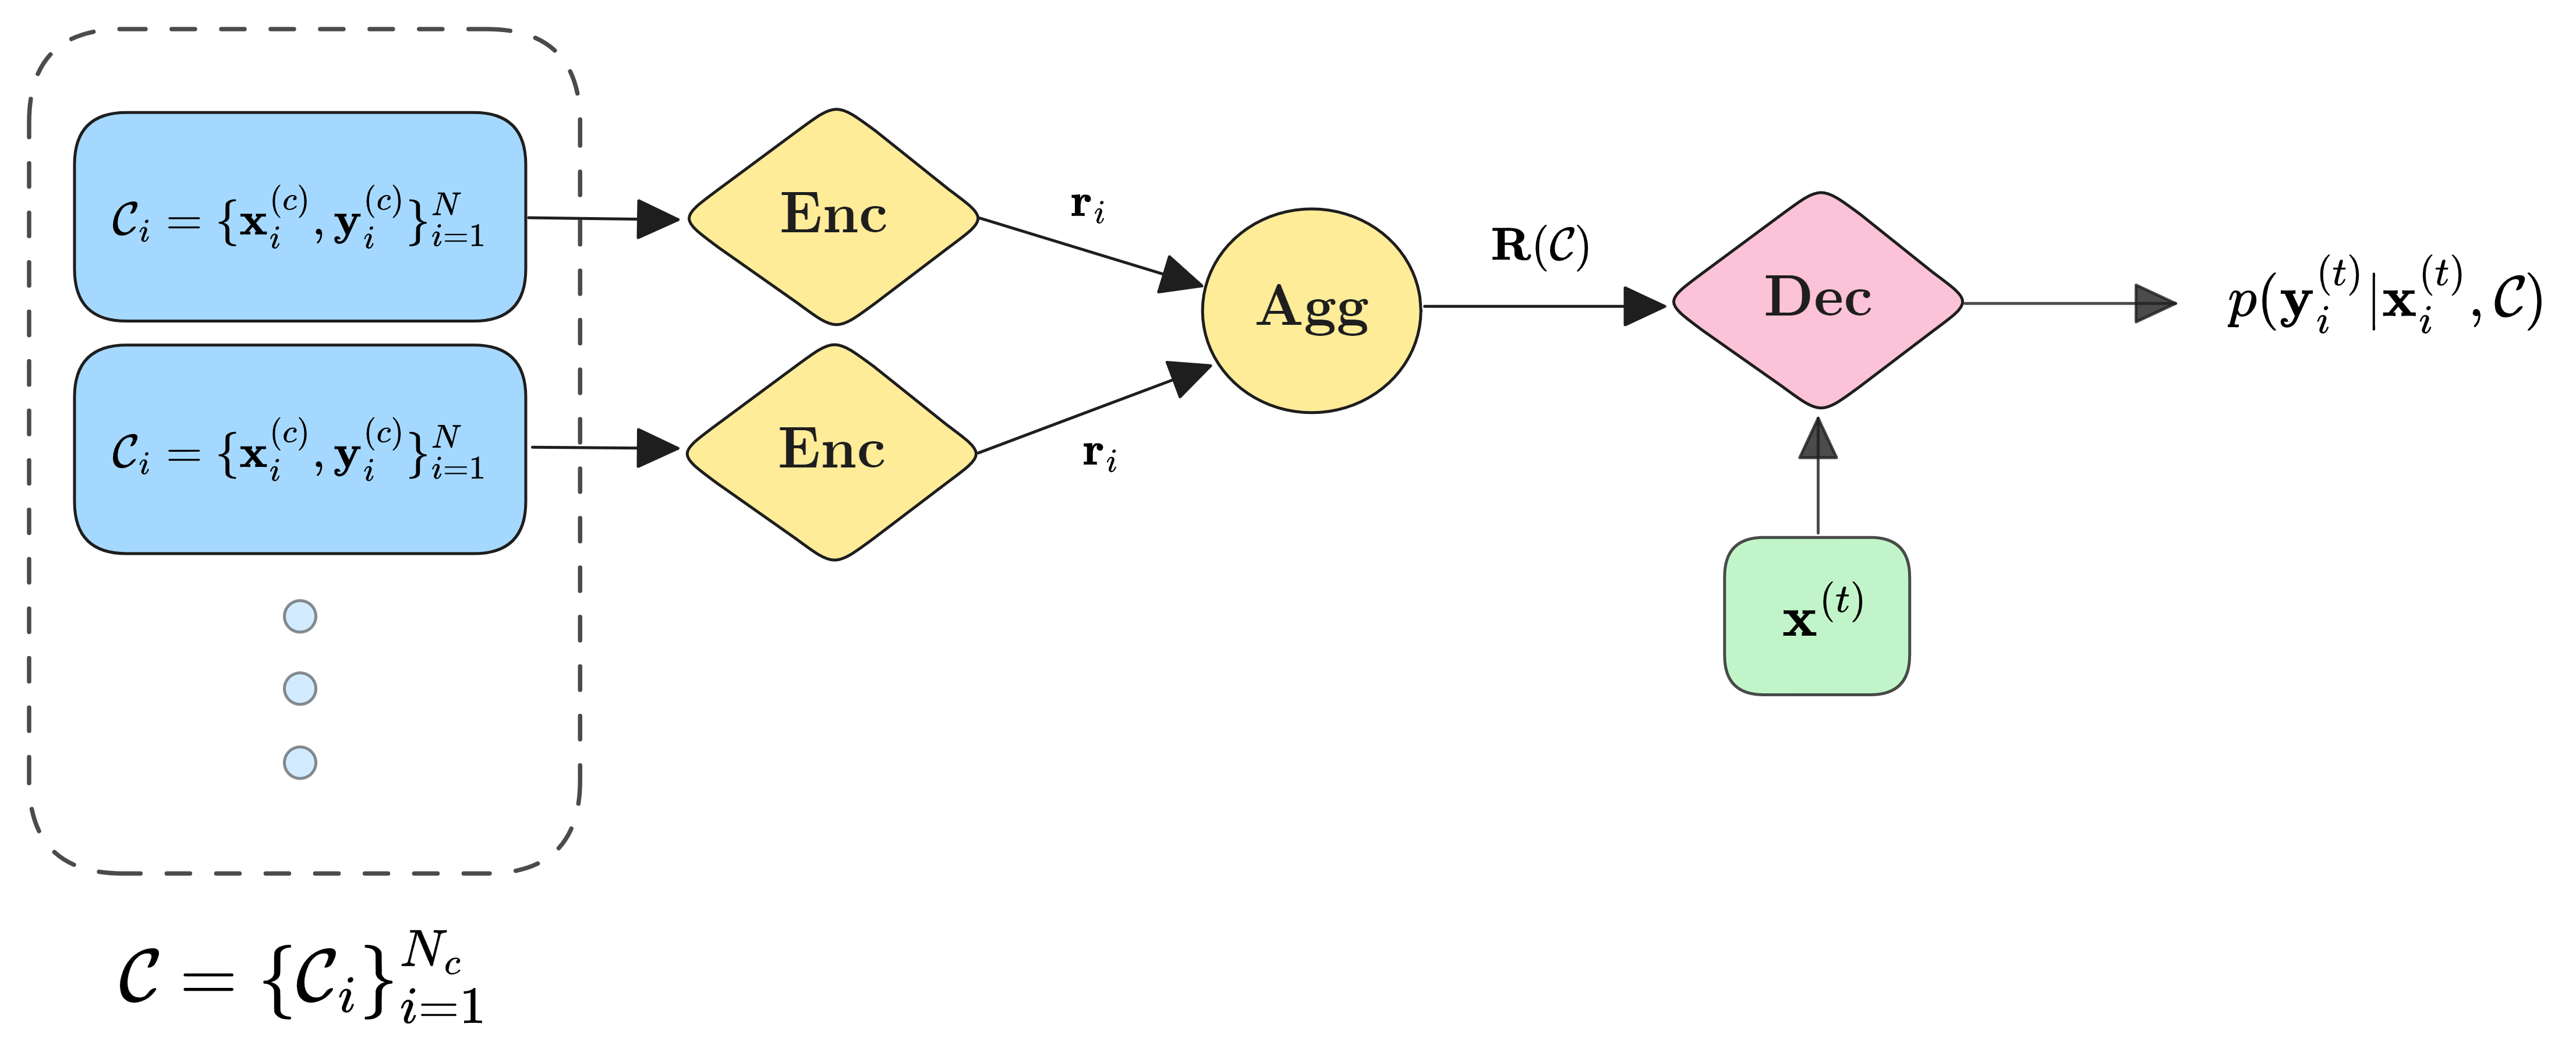
\includegraphics[height=0.3\textwidth]{./cnp.png}
	\caption{CNP Architecture}
	\label{fig:cnp-architecture}
\end{figure}




\subsection{Conditonal Neural Processes}

Conditional Neural Processes (CNPs) \cite{garnelo2018conditional} was one of the two original Neural Processes introduced by Garnelo et al. in 2018. Using the architecture framework described above, CNPs can be described as follows.

\begin{align*}
    \text{Enc}_{\theta_e} &= \text{MLP}_{\theta_e} \\
    \text{Agg} &= \text{Sum} \\
    \text{Dec}_{\theta_d}  &= \text{MLP}_{\theta_d} 
\end{align*}

The encoding and summation is an implementation of the `DeepSet' architecture \cite{zaheer2018deep} which is a neural network that is \textbf{Permutation Invariant} (PI) due to the summation operation. This means that the order of the input does not matter. 


CNPs make the strong assumption that the posterior distribution \emph{factorizes} over the target points. This means that the posterior distribution over the target points is independent of each other. 

\begin{align}
    p(\bm{y}\isup{t} | \bm{x}\isup{t}, \mathcal{C}) &\stackrel{(a)}{=} \prod_{i=1}^{N_t} p({y}_i\isup{t} | {x}_i\isup{t}, \bm{R}(\mathcal{C})) \\ &\stackrel{(b)}{=}
    \prod_{i=1}^{N_t} \mathcal{N}({y}_i\isup{t} | \mu_i, \sigma_i^2) \\&\stackrel{(c)}{=} \mathcal{N}(\bm{y}\isup{t} | \bm{\mu}(\bm{x}\isup{t}, \mathcal{C}), \bm{\Sigma}(\bm{x}\isup{t}, \mathcal{C}))
\end{align}

The benefit of this factorization assumption (a) is that the model can scale linearly with the number of target points with a tractable likelihood. However, this assumption means
\textbf{CNPs are unable to generate coherent sample paths, they are only able to produce distributions over the target points.} Furthermore, we need to select a marginal likelihood for the distribution (b) which is usually a Heteroscedastic Gaussian Likelihood (Gaussian with a variance that varies with the input) \cite{garnelo2018conditional}. This also adds a further assumption as we have to select a likelihood for the distribution which may not be appropriate for the data we are modeling.

Since the product of Gaussians is a Gaussian (c) the model learns a mean and variance for each target point (though typically we learn the log variance to ensure it is positive), in this way, the model decoder can be interpreted as outputting a function of mean and variance for each target point.

As the likelihood is a Gaussian, the model can be trained using simple maximum likelihood estimation (MLE) by minimizing the negative log-likelihood (NLL) of the target points.


\subsection{Latent Neural Processes}

Neural Processes better named `Latent Neural Processes' are an extension of CNPs that can generate coherent sample paths and are not restricted to a specific likelihood. They can do this by learning a latent representation of the context set $\mathcal{C}$ which is then used to condition the decoder. We will call this latent representation $\mathbf{z}$ (instead of $\bm{R}$) to avoid confusion with the non-latent global representation $\bm{R}$ used in CNPs).

The encoder learns a \emph{distribution} over the latent representation $\mathbf{z}$ of the context set $\mathcal{C}$. Then the decoder learns a distribution over the target outputs $\bm{y}\isup{t}$ conditioned on the latent representation $\mathbf{z}$ and the target inputs $\bm{x}\isup{t}$.

\begin{align*}
    p(\mathbf{z} | \mathcal{C}) &= \text{Enc}_\theta(\mathcal{C})\\ p(\bm{y}\isup{t} | \bm{x}\isup{t}, \mathbf{z}) &= \text{Dec}_\theta(\bm{x}\isup{t}, \mathbf{z})
\end{align*}

The full model is shown in Figure \ref{fig:lnp-architecture}.

\begin{figure}[H]
	\centering
	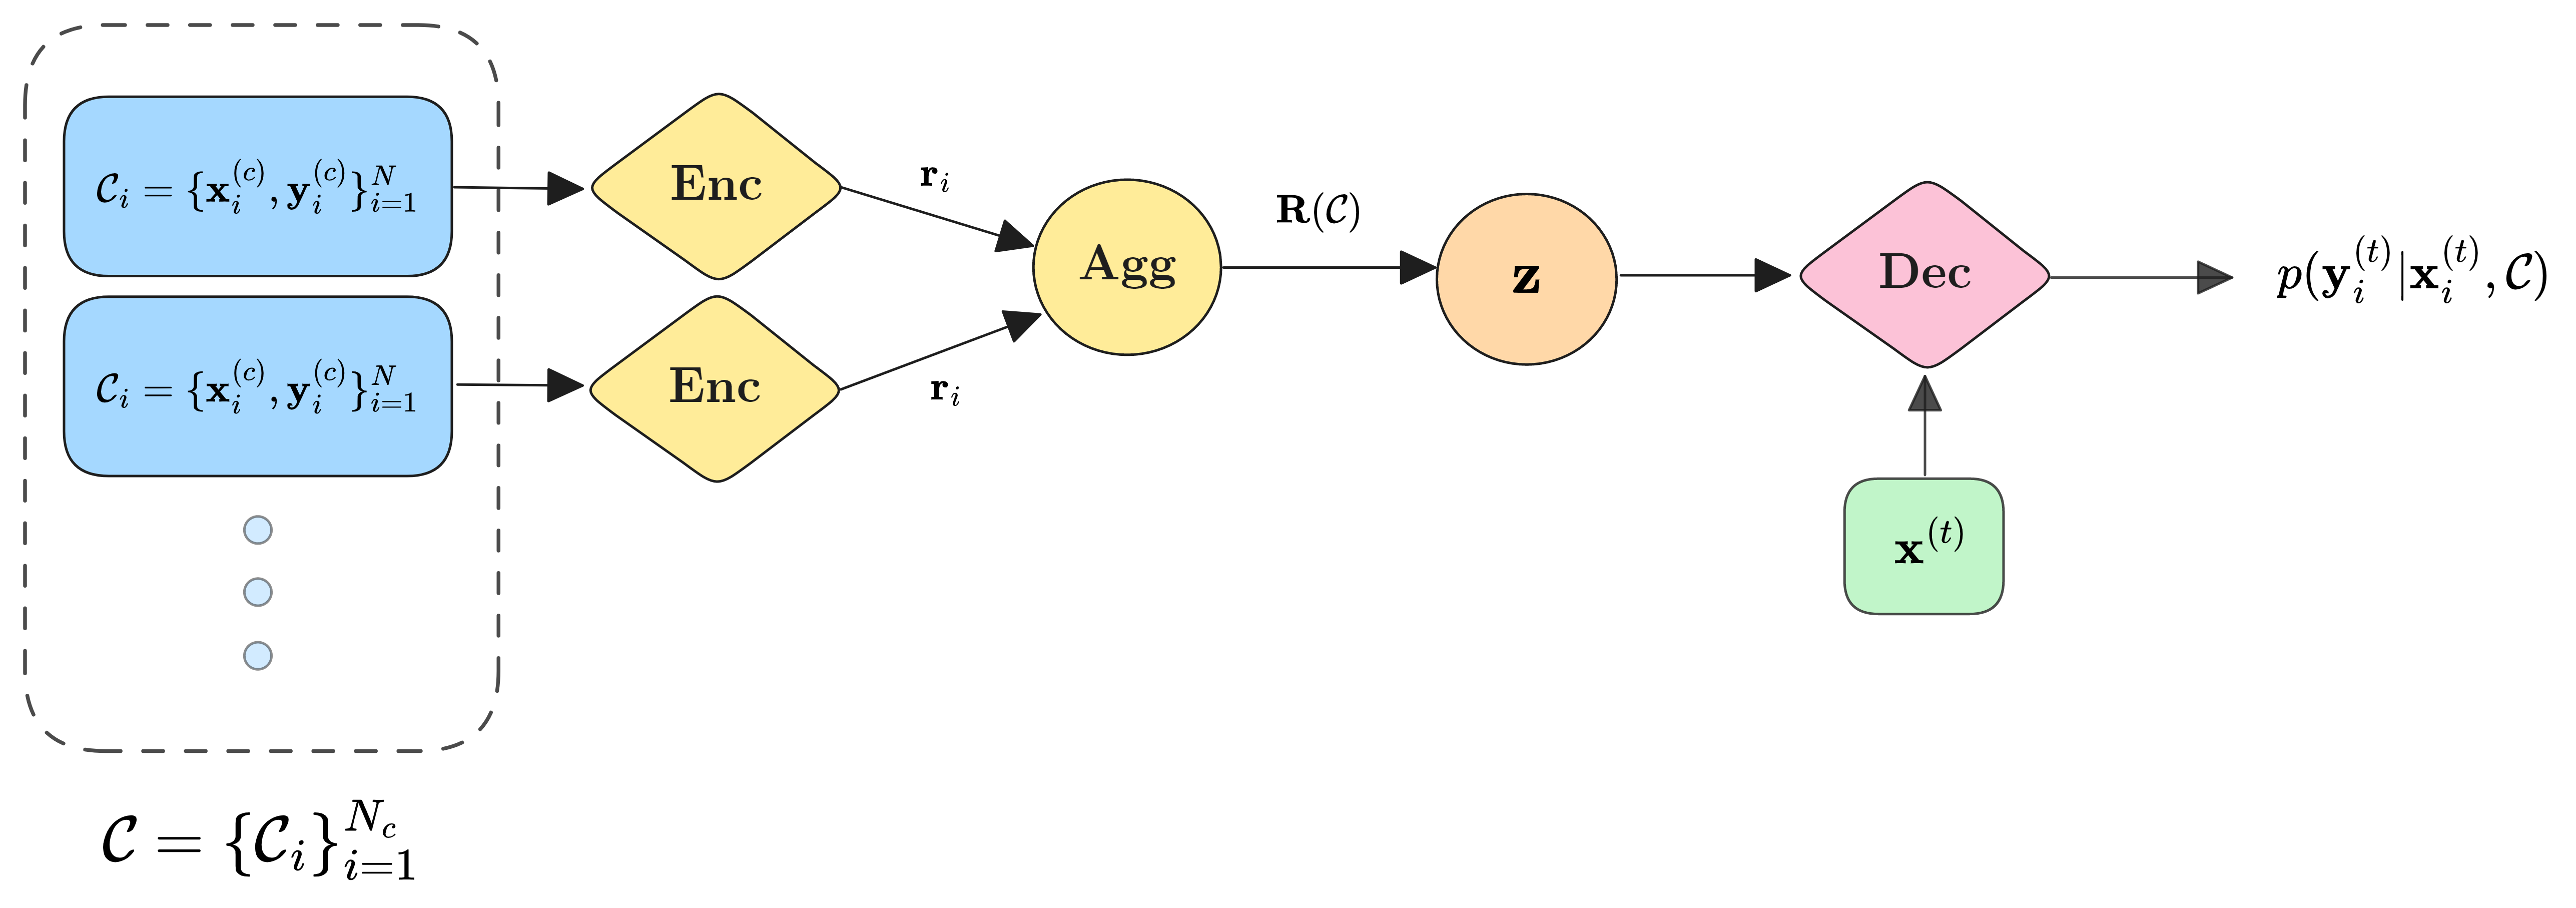
\includegraphics[height=0.3\textwidth]{./lnp.png}
	\caption{LNP Architecture}
	\label{fig:lnp-architecture}
\end{figure}

The likelihood of the target points is then given by the marginal likelihood of the latent representation $\mathbf{z}$.

\begin{align}
    p(\bm{y}\isup{t} | \bm{x}\isup{t}, \mathcal{C}) &=  \int p(\mathbf{z} | \mathcal{C}) p(\bm{y}\isup{t} | \bm{x}\isup{t}, \mathbf{z})  d\mathbf{z}
    \\ &\stackrel{(a)}{=} \int p(\mathbf{z} | \mathcal{C}) \left(\prod_{i=1}^{N_t} p({y}_i\isup{t} | {x}_i\isup{t}, \mathbf{z})\right)  d\mathbf{z}
    \\ &\stackrel{(b)}{=} \int p(\mathbf{z} | \mathcal{C}) \left(\prod_{i=1}^{N_t} \mathcal{N}({y}_i\isup{t} | \mu_i, \sigma_i^2)\right)  d\mathbf{z}
\end{align}

We can see that we express the conditional distribution over the target points conditioned on the latent representation $\mathbf{z}$ as a factorized (a) product of Gaussians (b), this may seem like we are making the same factorization assumption as CNPs. However, the difference is that we are not making this assumption conditioned on the latent variable instead of the context set. This integral models an \emph{infinite mixture} of Gaussians which allows us to model \emph{any} distribution over the target points.  The downside is that the likelihood is intractable and we need to use approximate inference methods such as Variational Inference (VI) or Sample Estimation using Monte Carlo (MC) methods to train the model which typically leads to biased estimates of the likelihood with high variance, thus we require more samples to train the model.


\section{Neural Processes vs Gaussian Processes}

\todo{HERE}

% From this, it is clear that NPs achieve a \emph{prediction} map, $\pi$ which maps the context set to the target set into a posterior distribution over the outputs. 

% \begin{equation}
%     \pi: \mathcal{C} \times \mathcal{X}\isup{t} \rightarrow \mathcal{P}(\mathcal{Y})
% \end{equation}


% This illustrates the similarity to Gaussian Processes (GP) \cite{books/lib/RasmussenW06} which perform the same underlying task of predicting the outputs of a target set conditioned on a context set. The difference is that GPs use a kernel function to compute the covariance between the context and target sets whereas NPs use a neural network to compute the covariance.

% \begin{align}
%     &\text{GP}: \pi \rightarrow \mathcal{N}(m(
%     \mathcal{C}, \bm{x}\isup{t})
%     ), k(\bm{x}\isup{c}, \bm{x}\isup{t})) \\
%     &\text{NP}: \pi \rightarrow \text{Dec}_\theta(\bm{x}\isup{t},  
%     \text{Agg}(\{ \text{Enc}_\theta(\mathcal{C}_i) \}_{i=1}^D))
% \end{align}


\section{Performance of Vanilla NP}

Whilst Neural Processes are very flexible and have the ability to scale, in reality due to the simple archiecture of the encoding and aggregation stage, they are unable to perform effectively in more complicated and higher dimensional data. This is because the model is unable to learn a good representation of the context set using a simple MLP and summation operation. 

The benefit of the NP is we can replace the encoder and decoder with more powerful models such as Convolutional Neural Networks (CNNs) or Transformers to learn a better representation of the context set. This allows us to scale the model using well known architectures that have been shown to perform well on a variety of tasks and at scale. Both CNN and Transformer based NPs are bound to have their unique advantages and disadvantages which we will explore in the following chapters by firstly exploring the Convolutional Neural Process (ConvCNP) and then the Transformer Neural Process (TNP).

% \ifSubfilesClassLoaded{%
%     \printbibliography{}
% }{} 


\end{document}